\clearpage
\phantomsection

\setcounter{chapter}{1}
\chapter[{CƠ SỞ LÝ THUYẾT}]{Thuật toán YOLO}

\section{Phần mềm GNU Radio và thiết bị vô tuyến định nghĩa bằng phần mềm SDR}

\subsection{Phần mềm GNU Radio}

\renewcommand{\labelitemi}{$-$}
\begin{itemize}
\item Waveform Generators 
	\begin{itemize}
		\item[$\diamond$] Signal Source (e.g. Sine, Square, Saw Tooth,...)
		\item[$\diamond$] Noise Source
		\item[$\diamond$] Constant Source
	\end{itemize}
\item Modulator
	\begin{itemize}
		\item[$\diamond$] AM Demod
		\item[$\diamond$] Continuous Phase Modulation
		\item[$\diamond$] PSK Mod / Demod
		\item[$\diamond$] GFSK Mod / Demod
		\item[$\diamond$] QAM Mod / Demod
		\item[$\diamond$] WBFM / NBFM Receive
		\item[$\diamond$] DVB-T / DVB-T2
		\item[$\diamond$] CDMA \cite{Kavitha2015}
		\item[$\diamond$] OFDM \cite{Bloessl2013}
	\end{itemize}
\item  Channel Models 
	\begin{itemize}
		\item[$\diamond$] Channel Model
		\item[$\diamond$] Fading Model
		\item[$\diamond$] Frequency Selective Fading Model
	\end{itemize}
\item Filters
	\begin{itemize}
		\item[$\diamond$] Low / High Pass Filter
		\item[$\diamond$] Band Pass / Reject Filter
		\item[$\diamond$] IIR Filter
		\item[$\diamond$] Decimating FIR Filter
		\item[$\diamond$] Hilbert
		\item[$\diamond$] Root Raised Cosine Filter
		\item[$\diamond$] FFT Filter
	\end{itemize}
\item Fourier Analysis 
	\begin{itemize}
		\item[$\diamond$] FFT
		\item[$\diamond$] FLL Band-Edge
		\item[$\diamond$] Rational Resampler (Synchronizers)
		\item[$\diamond$] PN Correlator
	\end{itemize}
\end{itemize}

Giao diện cho người dùng thông thường là GNU Radio Companion (GRC) được hiển thị như hình \ref{fig:GNURadio}. Với giao diện khá tương đồng với Matlab Simulink, gồm các khối nguồn, xử lý tín hiệu, hiển thị, widget,… dễ dàng chọn lựa, tùy chỉnh và kết nối với nhau thành flow-graph. Tất cả được GRC biên dịch ra file python và đẩy cho GNU Radio xử lý và hiển thị kết quả dựa trên QT GUI (QT Toolkit), hoặc Wx GUI (WxPython, tuy nhiên Wx Python đã bị xóa bỏ ở phiên bản GNU 3.8 do tốc độ đáp ứng chậm).

\begin{figure} [!h]
	\centering
	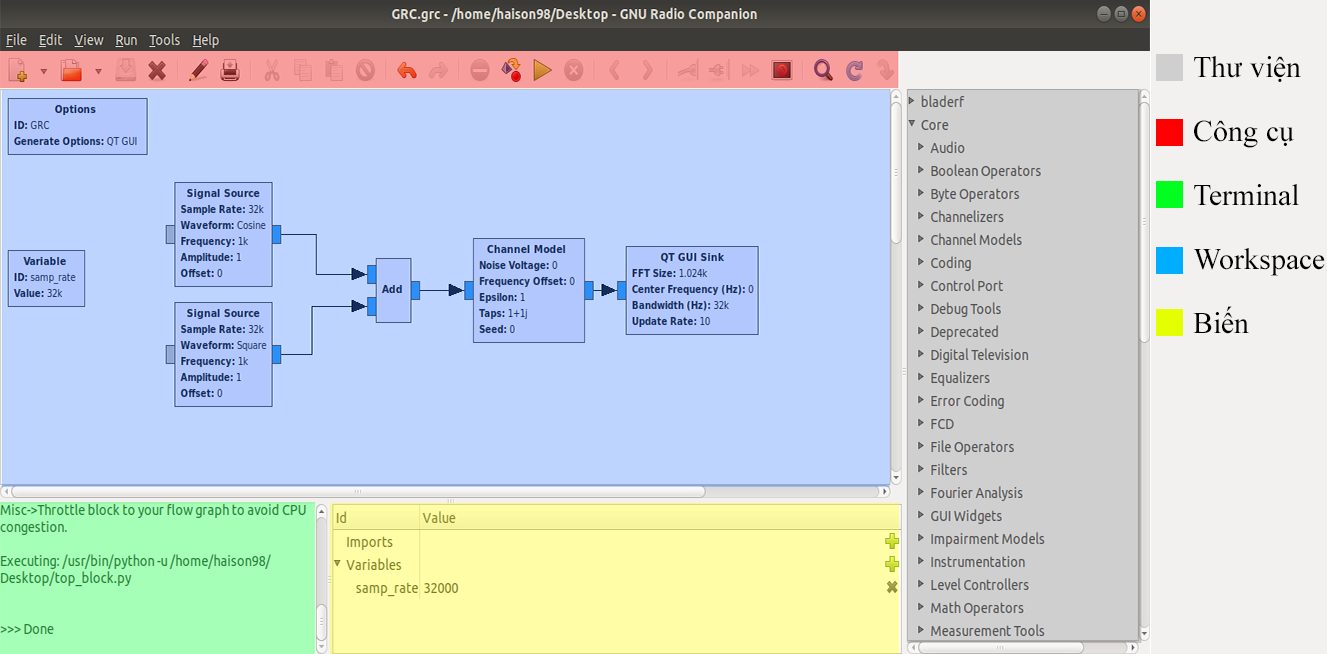
\includegraphics[width=1\linewidth]{figures/GNURadio1.png}
	\caption{Giao diện GNU Radio Companion}
	\label{fig:GNURadio}
\end{figure}

GNU Radio được viết hoàn toàn bằng ngôn ngữ C++ để đảm bảo hiệu năng, tuy nhiên người dùng vẫn có thể sử dụng Python để viết các khối do GNU Radio sử dụng SWIG để liên kết C++ với các ngôn ngữ bậc cao mà ở đây là Python. Hình \ref{fig:SWIG} mô tả cách thức vận hành của GNU Radio và cách nó liên kết với thiết bị SDR.

\begin{figure} [!htb]
	\centering
	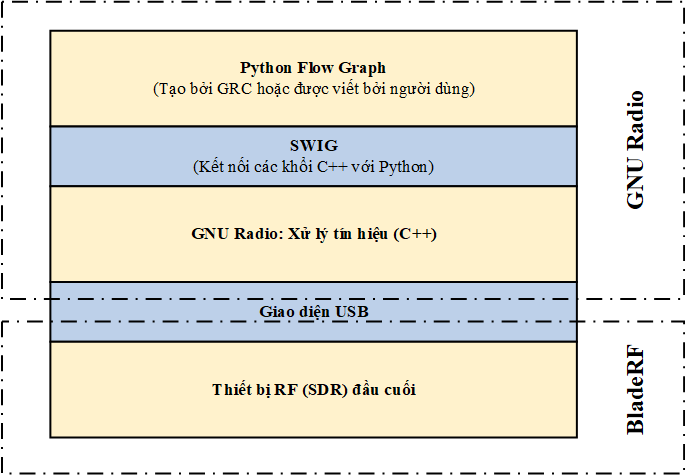
\includegraphics[width=0.9\linewidth]{figures/SWIG.png}
	\caption{Sơ đồ làm việc của GNU Radio}
	\label{fig:SWIG}
\end{figure}

Các luồng dữ liệu trong GNU Radio đi qua các khối thực thi được phân chia rõ ràng về kiểu dữ liệu như trên hình \ref{fig:colormapping} và độ dài của vector dữ liệu như hình \ref{fig:streamdata}, chỉ khi chúng khớp nhau, GRC thông báo hợp lệ thì chương trình mới có thể chạy. Điều này có được là do ngay trong việc khởi tạo khối, các thông số trên đã được định sẵn để đảm bảo việc xử lý tín hiệu là đúng với mục đích ban đầu của khối.

\begin{figure}[!h]
%\hfill
\centering
\subfigure[Mã màu của các kiểu dữ liệu]{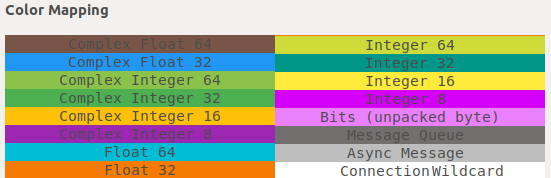
\includegraphics[width=0.9\linewidth]{figures/colormapping.png}\label{fig:colormapping}}
\hfill
\subfigure[Luồng dữ liệu qua các khối xử lý]{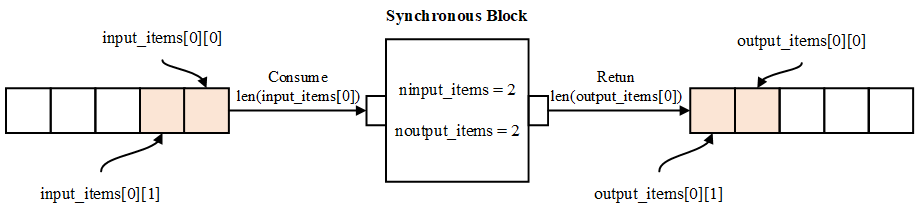
\includegraphics[width=0.9\linewidth]{figures/streamdata.png}\label{fig:streamdata}}
\hfill
\caption{Kiểu dữ liệu và xử lý tín hiệu trong GNU Radio}
\end{figure}

Đối với các nhà phát triển muốn tạo thêm các khối thực hiện các chức năng đặc biệt, GNU Radio cung cấp khả năng tương thích với cả C++ và Python. Bảng \ref{methodGNURadio} dưới đây so sánh tính năng của các phương pháp lập trình khối trong GNU Radio.

\begin{table}[!h]
	\caption{Các phương pháp sử dụng GNU Radio}
	\resizebox{1\hsize}{!} {
		\begin{tabular}{|l|l|l|}
			\hline
			\multicolumn{1}{|c|}{\multirow{2}{*}{\textbf{GNU Radio Companion}}} & \multicolumn{1}{c|}{\multirow{2}{*}{\textbf{C++}}} & \multicolumn{1}{c|}{\multirow{2}{*}{\textbf{Python}}} \\
			\multicolumn{1}{|c|}{} & \multicolumn{1}{c|}{} & \multicolumn{1}{c|}{} \\ \hline
			&  &  \\
			Dễ dàng và trực quan. & Đầy đủ các tùy chỉnh. & Đầy đủ các tùy chỉnh. \\
			&  &  \\ \hline
			&  &  \\
			\begin{tabular}[c]{@{}l@{}}Tạo flow-graph bằng cách kết nối và\\ tinh chỉnh các khối có sẵn trong GRC.\end{tabular} & Tốc độ thực thi nhanh. & \begin{tabular}[c]{@{}l@{}}Lập trình nhanh chóng\\ (Numpy, Scipy,...)\end{tabular} \\
			&  &  \\ \hline
			&  &  \\
			& Thực hiện tốt các hệ truyền thông thời gian thực. & \begin{tabular}[c]{@{}l@{}}Tốt trong việc thực hiện các\\ thực nghiệm nhanh chóng.\end{tabular} \\
			&  &  \\ \cline{2-3} 
			&  &  \\
			& Độ phức tạp và thời gian lập trình lâu. &  \\
			&  &  \\ \cline{2-2}
			&  &  \\
			& Kết nối với Python bằng SWIG. &  \\
			&  &  \\ \hline
	\end{tabular} }
	\label{methodGNURadio}
\end{table}

%\begin{figure} [!h]
%	\centering
%	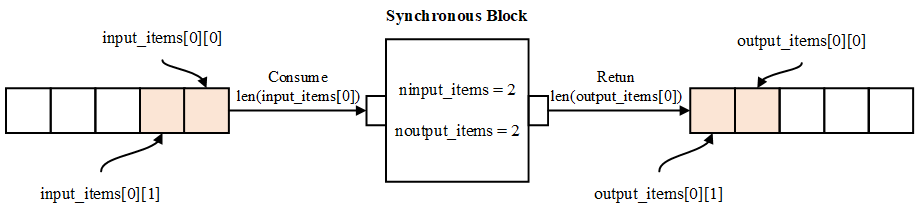
\includegraphics[width=1\linewidth]{figures/streamdata.png}
%	\caption{Luồng dữ liệu qua các khối xử lý trong GNU Radio}
%	\label{fig:streamdata}
%\end{figure}

\subsection{Thiết bị vô tuyến định nghĩa bằng phần mềm SDR}

Vô tuyến định nghĩa bằng phần mềm (Software Define Radio) là một hệ thống truyền thông vô tuyến được thực hiện chủ yếu bằng phần mềm trên máy tính cá nhân hoặc hệ thống nhúng. Một SDR cơ bản bao gồm máy tính có sound card  hoặc thiết bị chuyển đổi tương tự sang số (ADC) cùng thiết bị chuyển đổi số sang tương tự (DAC) và đầu cuối cao tần để thu phát tín hiệu, mô tả khái quát ở hình \ref{fig:structSDR}. Phần xử lý tín hiệu hầu hết được thực hiện bởi bộ xử lý đa năng (GPP) thay vì phần cứng chuyên dụng (mạch điện tử). Với thiết kế này một thiết bị SDR có thể truyền nhận được tín hiệu ở nhiều tần số,  loại điều chế khác nhau chỉ dựa trên phần mềm sử dụng.

\begin{figure} [!htb]
	\centering
	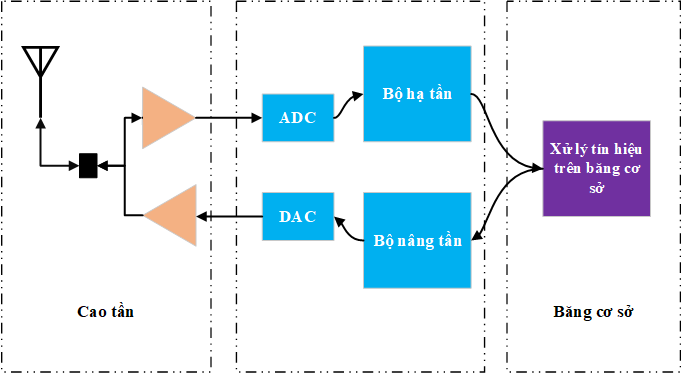
\includegraphics[width=1\linewidth]{figures/structSDR.png}
	\caption{Sơ đồ khối phần cứng hệ thống SDR}
	\label{fig:structSDR}
\end{figure}

Software Define Radio được sử dụng trong các ứng dụng quân sự \cite{Bergstrom2002} và trong viễn thông di động \cite{VanRijsbergen, Gomez-Miguelez2016}, cả hai đều có thể sử dụng nhiều giao thức vô tuyến và đáp ứng thời gian thực. Về lâu dài, SDR được mong đợi sẽ trở thành công nghệ thống trị trong truyền thông vô tuyến bằng cách kết hợp với Anten định nghĩa bằng phần mềm (Software Define Antennas) tạo thành vô tuyến nhận thức (Cognitive Radio).

Với tên ban đầu máy thu kỹ thuật số (Digital Receiver) được tạo ra vào năm 1970 bởi một nhà nghiên cứu thuộc bộ quốc phòng Hoa Kỳ, từ năm 1990 đến 1995, ứng dụng trong dự án SpeakEasy \cite{Fakhrian2012}, một chương trình cho các đài phát thanh điều khiển không quân mặt đất chiến thuật của không quân Hoa Kỳ có thể hoạt động từ 2 MHz đến 2 GHz. Thuật ngữ Software Define Radio do Stephen Blust đặt ra và đề xuất tại Modular Multifunction Information Transfer Systems năm 1996. Tiếp tục được nghiên cứu và phát triển liên tục sau đó, đến nay đã có nhiều sản phẩm thương mại SDR đã bán ra trên toàn cầu cho mục đích quân sự, nghiên cứu, giảng dạy hay ứng dụng vào sản phẩm truyền thông không dây thực tế. Có thể kể đến trong quân sự, dự án Joint Tactical Radio System (JTRS) \cite{Feickert2005} sản xuất bộ đàm cung cấp liên lạc linh hoạt và có thể tương tác, nhưng do vấn đề chi phí cao hơn so với việc sử dụng các linh kiện chuyên dụng cho một mục đích nên chưa được sử dụng rộng rãi. Tuy nhiên, tính linh hoạt của SDR có thể là chìa khóa cho truyền thông vô tuyến trong tương lai, một khi chi phí cố định để sản xuất một SDR đã giảm đủ để vượt qua chi phí thiết kế lại các hệ thống sử dụng linh kiện điện tử cho một mục đích.

\begin{figure} [!htb]
	\centering
	\includegraphics[width=0.5\linewidth]{figures/commonSDR.png}
	\caption{Các thiết bị SDR thông dụng}
	\label{fig:commonSDR}
\end{figure}

Các ứng dụng trong giảng dạy và nghiên cứu với SDR thông dụng hơn, với rất nhiều thiết bị SDR ở nhiều mức giá và mục đích khác nhau (hình \ref{fig:commonSDR}). Từ các thiết bị giá rẻ chỉ 22 \$ như DVB-T USB dongles sử dụng IC điều khiển Realtek RTL2832U, và Rafael Micro R820T làm bộ chỉnh tần số, thiết bị chỉ thực hiện chức năng thu tín hiệu, có thể hoạt động trong dải từ 500 kHz đến 1,75 GHz để thu FM, DVB-T, GSM,... Với các nghiên cứu chuyên sâu hơn Universal Software Radio Peripheral (USRP) là lựa chọn tốt với dải thu siêu cao tần lên đến 6 GHz băng thông rộng 200 MHz cùng khả năng MIMO được tích hợp sẵn.

\section{Phần cứng và phần mềm của BladeRF}

\subsection{BladeRF x115}

Trong nghiên cứu này  sử dụng các Kit SDR là BladeRF x115 của Nuand, ra mắt năm 2013, được tích hợp nhiều công nghệ mới: hỗ trợ truyền nhận đồng thời (full duplex), bộ ADC, DAC tốc độ cao, khả năng lập trình FPGA, tương thích giao diện USB 3.0, cổng kết nối mở rộng (GPIO), MIMO,... Các thông số chi tiết ở bảng \ref{parabladeRF}.

% Please add the following required packages to your document preamble:
% \usepackage[table,xcdraw]{xcolor}
% If you use beamer only pass "xcolor=table" option, i.e. \documentclass[xcolor=table]{beamer}
%\begin{table}[!htb]
%\resizebox{1\hsize}{!} {
%\begin{tabular}{lcccc}
%\hline
%\rowcolor[HTML]{FFECEA} 
%Thông Số & Nhỏ nhất & Thông thường & Lớn nhất & Đơn vị \\ \hline
%\rowcolor[HTML]{EFEFEF} 
%\multicolumn{5}{l}{\cellcolor[HTML]{EFEFEF}Thông số kỹ thuật RF} \\ \hline
%ADC/DAC Sample Rate & 0.16 &  & 40 & MHz \\ \hline
%ADC/DAC Resolution &  & 12 &  & bits \\ \hline
%VCTCXO Accuracy &  & 1 &  & ppm \\ \hline
%RF Tuning Range & 300 &  & 3 800 & MHz \\ \hline
%RF Bandwidth Filter & 1.5 &  & 28 & MHz \\ \hline
%CW Output &  & +6 &  & dBm \\ \hline
%\rowcolor[HTML]{EFEFEF} 
%\multicolumn{5}{l}{\cellcolor[HTML]{EFEFEF}Thông số kỹ thuật FPGA} \\ \hline
%Logic Elements &  &  & 114 480 & LE \\ \hline
%Embedded 18x18 Multipliers &  &  & 266 &  \\ \hline
%BRAM &  &  & 3 888 & kbits \\ \hline
%\rowcolor[HTML]{EFEFEF} 
%\multicolumn{5}{l}{\cellcolor[HTML]{EFEFEF}Thông số vật lý} \\ \hline
%Kích thước &  & 8.7 x 13.1 x 1.8 &  & cm \\ \hline
%Cân nặng &  & 80 &  & g \\ \hline
%Nhiệt độ làm việc & 0 &  & 70 & $^{\circ}$C \\ \hline
%\end{tabular} 
%}
%\caption{Thông số kỹ thuật của BladeRF x115}
%\label{parabladeRF}
%\end{table}

\begin{table}[!htb]
\caption{Thông số kỹ thuật của BladeRF x115}
\resizebox{1\hsize}{!} {
\begin{tabular}{|l|c|c|c|c|} 
\hline
\rowcolor[rgb]{1,0.925,0.918} Thông Số & Nhỏ nhất & Thông thường     & Lớn nhất & Đơn vị        \\ 
\hline
\multicolumn{5}{|l|}{{\cellcolor[rgb]{0.937,0.937,0.937}}Thông số kỹ thuật RF}                  \\ 
\hline
ADC/DAC Sample Rate                    & 0,16     &                  & 40       & MHz           \\ 
\hline
ADC/DAC Resolution                     &          & 12               &          & bits          \\ 
\hline
VCTCXO Accuracy                        &          & 1                &          & ppm           \\ 
\hline
RF Tuning Range                        & 300      &                  & 3 800    & MHz           \\ 
\hline
RF Bandwidth Filter                    & 1,5      &                  & 28       & MHz           \\ 
\hline
CW Output                              &          & +6               &          & dBm           \\ 
\hline
\multicolumn{5}{|l|}{{\cellcolor[rgb]{0.937,0.937,0.937}}Thông số kỹ thuật FPGA}                \\ 
\hline
Logic Elements                         &          &                  & 114 480  & LE            \\ 
\hline
Embedded 18x18 Multipliers             &          &                  & 266      &               \\ 
\hline
BRAM                                   &          &                  & 3 888    & kbits         \\ 
\hline
\multicolumn{5}{|l|}{{\cellcolor[rgb]{0.937,0.937,0.937}}Thông số vật lý}                       \\ 
\hline
Kích thước                             &          & 8,7 x 13,1 x 1,8 &          & cm            \\ 
\hline
Cân nặng                               &          & 80               &          & g             \\ 
\hline
Nhiệt độ làm việc                      & 0        &                  & 70       & $^{\circ}$C   \\
\hline
\end{tabular}
}
\label{parabladeRF}
\end{table}

Cấu hình bên trong của BladeRFx115 biểu diễn trên hình \ref{fig:structbladeRF}, các thành phần chính bao gồm: 

\begin{figure} [!htb]
	\centering
	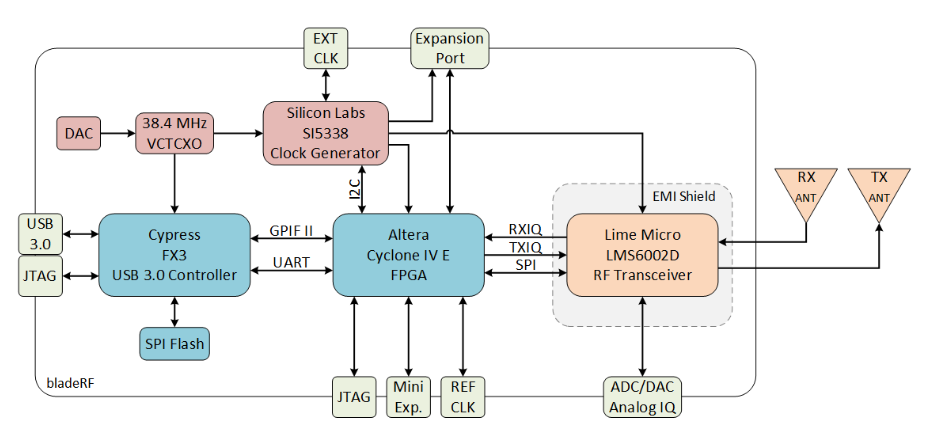
\includegraphics[width=1\linewidth]{figures/structbladeRF.png}
	\caption{Cấu hình của BladeRF x115}
	\label{fig:structbladeRF}
\end{figure}

\begin{itemize}
	\item	Altera Cyclone IV EP4CE15 FPGA: thành phần xử lý trung tâm của BladeRF, có thể lập trình lại qua cổng JTAG.
	\item 	Lime Micro LMS6002D RF Transceiver: IC thu phát cao tần có thể lập trình, hoạt động trong dải 300 MHz đến 3,8 GHz, trên cả băng tần được cấp phép và không được cấp phép và với bất cứ tiêu chuẩn truyền thông không dây nào. Các bộ ADC, DAC 12 bits truyền trực tiếp mẫu đến FPGA. Tích hợp sẵn LNA, PA, bộ trộn TX/RX, bộ lọc TX/RX, ...
	\item   Cypress FX3 USB 3.0 Controller: bộ điều khiển ngoại vi USB 3.0 tốc độ cao băng thông 5 Gbps, có cấu hình qua $\mathrm{GPIF^{TM} II}$. Là cầu nối giao tiếp giữa BladeRF và máy tính hay các thiết bị ngoại vi khác như SPI Flash.
	\item   SPI Flash: IC MX25U3235EM2I-10G cung cấp 32 Mb bộ nhớ Flash.
	\item   Silicon Labs Si5338 Clock Generator: bộ tạo xung đồng hồ chuẩn cho toàn BladeRF, giao tiếp với FPGA qua chuẩn I2C.
	\item 	VCTCXO: bộ tạo dao động tinh thể để bù cho nhiệt độ, được hiệu chuẩn ở mức sai số dưới 1 Hz trong 38,4 MHz.
	%\item 	SPI Flash: sử dụng IC MX25U3235EM2I-10G cung cấp 32Mb bộ nhớ Flash.
	\item 	Expansion port, EXT CLK, Mini Exp, REF CLK, JTAG, ADC/DAC Analog IQ: các cổng mở rộng để phục vụ từng mục đích chuyên biệt cho BladeRF.
\end{itemize}

\subsection{Phần mềm của BladeRF}

Dữ liệu đầu ra từ BladeRF truyền về máy tính là các mẫu IQ được lấy mẫu như hình \ref{fig:IQsample}, lưu ở chuẩn SC16Q11, khi đưa vào các khối trong GNU Radio sẽ chuyển đổi sang Complex Float32.

\begin{figure} [!h]
	\centering
	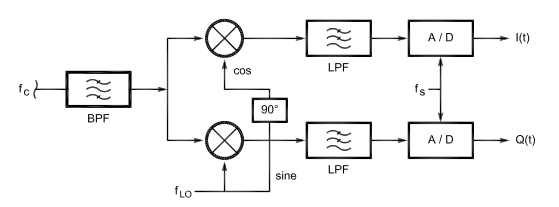
\includegraphics[width=1\linewidth]{figures/IQsample.png}
	\caption{Lấy mẫu IQ}
	\label{fig:IQsample}
\end{figure}

Để sử dụng dữ liệu đầu ra của BladeRF cho công việc xác định hướng sóng đến, cần phải viết thêm những khối OTT (Out Of Tree Modules) vào GNU Radio để đảm nhiệm việc xử lý tín hiệu. Có nhiều cách để tạo một khối OTT trên GNU Radio, đơn giản nhất là sử dụng ngay Python Block là một khối trong thư viện của GNU Radio, cho phép lập trình một khối mới ngay lập tức với ngôn ngữ Python, hình \ref{fig:pythonblock} là khối Python Block trên GRC và mã lập trình có sẵn bên trong khối. Tuy nhiên hạn chế ở hiệu năng và không thể tùy biến được nhiều và sâu cho khối, vì vậy chỉ nên sử dụng khi kiểm tra nhanh thuật toán. Một cách nữa do nhà phát hành cung cấp chính thức cho các nhà phát triển đó là công cụ gr\_modtool.
\newpage
\begin{figure}[!htb]
%\hfill
\subfigure[Khối Python Block trên GRC]{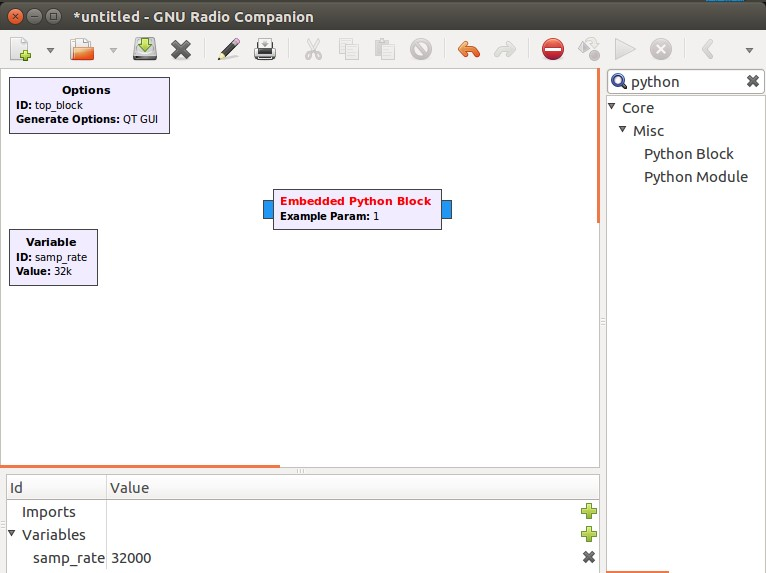
\includegraphics[width=0.49\linewidth]{figures/pythonblock.jpg}}
\hfill
\subfigure[Lập trình cho khối Python Block]{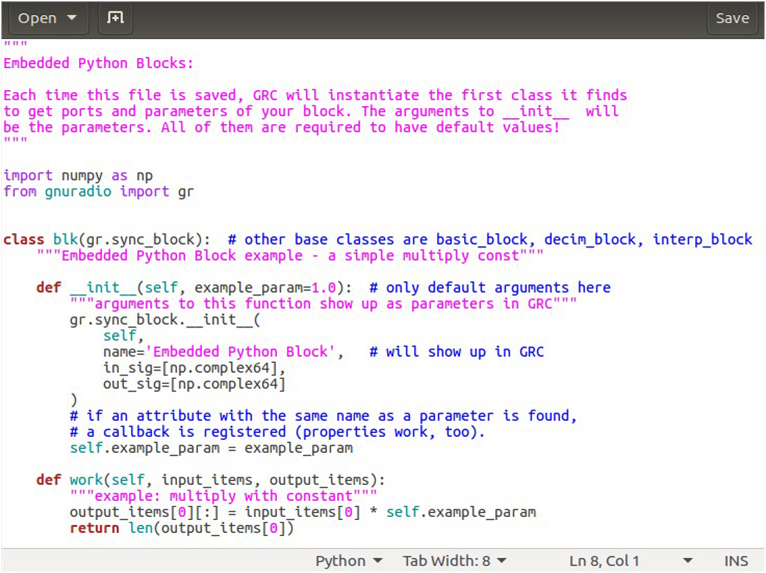
\includegraphics[width=0.49\linewidth]{figures/pythonblock2.jpg}}
\hfill
\caption{Tạo khối với Python Block trên GNU Radio}
\label{fig:pythonblock}
\end{figure}

Công cụ gr\_modtool được tích hợp sẵn vào GNU Radio từ năm 2010, sử dụng để tạo sẵn template các khối OTT với chức năng đa dạng cho người dùng, giúp bỏ qua các bước phải lặp đi lặp lại như: tạo các mã soạn sẵn, sửa makefile, ... Hỗ trợ lập trình khối cho GNU Radio với ngôn ngữ C++ và Python với liên kết bằng SWIG tích hợp sẵn, việc cài đặt các khối sau khi lập trình được thực  hiện tự động bằng CMAKE, hoàn toàn phù hợp cho cả người mới bắt đầu vào các mục đích nghiên cứu chuyên sâu. Hình \ref{fig:grmodtool} ví dụ một Module tạo bằng gr\_modtool chứa nhiều thư mục và file đã tạo sẵn, một Module có thể chứa nhiều khối OTT.

\begin{figure} [!h]
	\centering
	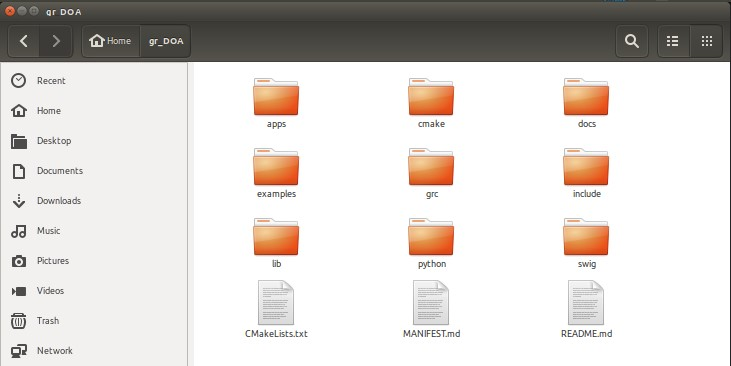
\includegraphics[width=1\linewidth]{figures/grmodtool.jpg}
	\caption{Module tạo bằng gr\_modtool}
	\label{fig:grmodtool}
\end{figure}

Tiếp theo, cần xác định loại khối cho các mục đích khác nhau, dưới đây là 4 loại khối được GNU Radio cung cấp:
\renewcommand{\labelitemi}{$-$}
\begin{itemize}
	\item Synchronous Blocks: Số mẫu đầu vào và đầu ra của khối là bằng nhau (1/1).
	\item Decimation Blocks: Cứ N mẫu đầu vào thì có 1 mẫu đầu ra (N/1).
	\item Interpolation Blocks: Cứ 1 mẫu đầu vào thì có M mẫu đầu ra (1/M).
	\item General Blocks: Tùy chỉnh tỷ lệ số mẫu đầu vào và đầu ra (N/M).
\end{itemize}

Việc cài đặt khối vào GNU Radio sau khi lập trình xong cũng rất đơn giản do sử dụng CMAKE, sau khi đã cài đặt, các khối OTT sẽ xuất hiện trong hộp thoại của GRC, dễ dàng chọn, tùy chỉnh thông số và kết nối với nhau.

\section{Triển khai hệ thống xác định hướng sóng đến trên hệ BladeRF}

Trên thực tế, việc xây dựng một hệ thống gồm nhiều thiết bị SDR mà ở đây là BladeRF để phục vụ cho việc xác định hướng sóng đến, yêu cầu hệ thu cần phải được đồng bộ hoàn toàn với nhau trước khi sử dụng dữ liệu của SDR để ước lượng DOA.

Trong phần này, để phù hợp với thực tế về số lượng SDR và phần cứng có sẵn, mảng anten thu sẽ chỉ gồm 2 phần tử BladeRF. Các bước đồng bộ dưới đây vẫn áp dụng được cho hệ nhiều phần tử BladeRF, tuy nhiên sẽ cần thêm các phần cứng chuyên dụng: bộ chia bù công suất, bộ chia giữ nguyên độ lệch pha, máy phát xung chuẩn. Chi tiết như sau: 

Không giống như dữ liệu lý tưởng khi mô phỏng, dữ liệu thực tế từ hệ SDR sẽ gặp các vấn đề cần phải được xử lý: xung đồng hồ chủ khác nhau; $\textrm{DC}_\textrm{offset}$ và cân bằng mẫu IQ cho các từng thiết bị SDR; việc truyền/nhận dữ liệu từ GNU Radio trên máy tính đến các SDR qua cổng USB thường không được thực hiện đồng thời, dẫn đến hiện tượng các các SDR bắt đầu chạy và gửi mẫu về ở các thời gian khác nhau, gây ra trễ mẫu ($\textrm{sample}_{\textrm{offset}}$) trên dữ liệu mảng thu; sai số trong thời gian lấy mẫu (\textrm{time sampling}); độ lệch pha giữa 2 tín hiệu ($\textrm{phase}_{\textrm{offset}}$) ở trạng thái ban đầu; cùng với vấn đề sai số ($f_{\textrm{offset}}$) trong tần số thu của từng SDR. Khi hiệu chỉnh hoàn tất, hệ SDR đồng bộ thì mới sử dụng được dữ liệu của chúng cho thuật toán DOA để ước lượng hướng sóng đến. Bảng \ref{tab:issue} bên dưới nêu ra các phương pháp được sử dụng để đồng bộ hệ BladeRF trong khóa luận và đưa thêm một số phương pháp khác có thể áp dụng cho các loại SDR khác.


\begin{sidewaystable}[htbp]
\centering
\caption{Phương pháp đồng bộ hệ BladeRF được sử dụng trong khóa luận}
%\begin{table}[!h]
\begin{tabular}{|l|l|l|}
	\hline
	\rowcolor[HTML]{FFECEA} 
	\multicolumn{1}{|c|}{\cellcolor[HTML]{FFECEA}\textbf{Vấn đề đồng bộ}} & \multicolumn{1}{c|}{\cellcolor[HTML]{FFECEA}\textbf{Phương pháp giải quyết được sử dụng}} & \multicolumn{1}{c|}{\cellcolor[HTML]{FFECEA}\textbf{Các phương pháp khác}} \\ \hline
	\begin{tabular}[c]{@{}l@{}}$\mathrm{DC}_\mathrm{offset}$\\ và cân bằng mẫu IQ\end{tabular} & \begin{tabular}[c]{@{}l@{}}Hiệu chỉnh bằng tính năng trong thư viện của BladeRF\\ có sẵn, và khối DC Blocker trên GNU Radio.\end{tabular} &  \\ \hline
	Xung đồng hồ chủ & \begin{tabular}[c]{@{}l@{}}Chia sẻ xung đồng hồ chủ (CLK) qua chân\\ SMB (System Management Bus) trên BladeRF.\end{tabular} & \begin{tabular}[c]{@{}l@{}}$\ast$ Sử dụng thêm phần cứng:\\ $-$ Silicon Labs SI5338 Clock Generator Evaluation Board, \\ sử dụng cùng loại IC SI5338 như trên BladeRF cho phép chia xung\\ tối đa đến 8 thiết bị khác.\end{tabular} \\ \hline
	$\mathrm{Sample}_\mathrm{offset}$ & Phân tích tương quan chéo của tín hiệu mảng thu. & \begin{tabular}[c]{@{}l@{}}$\ast$ Sử dụng thêm phần cứng: \\ $-$ Noise Source Card và tương quan chéo của nhiễu Gauss,\\ chuyển đổi qua lại giữa Noise Source Card và RF từ anten \\ qua giao tiếp I2C \cite{kerberos}.\\ $-$ Sử dụng chân MIMO có trên các SDR cao cấp (BladeRF, USRP), \\ trên BladeRF x115: chân J71 pin 4.\\ \\ $\ast$ Sử dụng phần mềm:\\ $-$ Sử dụng một kênh tham chiếu cố định (FM, DVB-T, GSM, ...)\\ được thực hiện trong dự án Multi-RTL: sử dụng kênh BCCH của \\ GSM để đồng bộ \cite{multi-rtl}.\end{tabular} \\ \hline
	$\textrm{Time sampling}$ & Do đã chia sẻ CLK nên bỏ qua công đoạn này. & \begin{tabular}[c]{@{}l@{}}$\ast$ Sử dụng thêm phần cứng:\\ $-$ Sử dụng chân J71 pin 4, tính năng Trigger trong $bladeRF-cli$\\ khóa xung lấy  mẫu của các BladeRF với nhau.\end{tabular} \\ \hline
	$f_\mathrm{offset}$ & Công cụ kalibrate-bladeRF do nhà sản xuất cung cấp. & \begin{tabular}[c]{@{}l@{}}$\ast$ Sử dụng thêm phần cứng:\\ $-$ Cấp tín hiệu chuẩn: 1 xung/giây hoặc 10 MHz ở mức điện áp 1,8 V \\ qua chân J71 pin 1 để hiệu chỉnh VCTCXO.\end{tabular} \\ \hline
	$\mathrm{Phase}_\mathrm{offset}$ & \begin{tabular}[c]{@{}l@{}}Sử dụng thuật toán MUSIC tìm độ lệch pha\\ giữa 2 tín hiệu.\end{tabular} & \begin{tabular}[c]{@{}l@{}}$\ast$ Sử dụng thêm phần cứng:\\ $-$ Sử dụng tín hiệu từ máy phát chuẩn như ở \cite{TravisFCollins}, cấp đến các SDR,\\ ước lượng độ lệch pha qua công thức: \\ \hspace{3cm} $\phi = tan^{-1} \left (\frac{Im (x(k))}{Re(x(k))} \right )$\\  với $Re$ và $Im$ lần lượt là phần thực và ảo của mẫu IQ. Sau đó, \\ bù thêm pha cho tín hiệu trễ pha: \\ \hspace{3cm} $\Delta \phi = \phi_1 - \phi_0 $\\ $ \hspace{3.2cm} \hat{\mathbf{x}}_1 = \mathbf{x}_1  e^{j \Delta \phi}$\end{tabular} \\ \hline
\end{tabular}
%\end{table}
\label{tab:issue}
\end{sidewaystable}
\newpage
Chi tiết các bước và kết quả đồng bộ hệ BladeRF x115 như sau:

\begin{itemize}
	\item[$\ast$] \textbf{Đồng bộ xung đồng hồ giữa các thiết bị SDR mảng thu}
\end{itemize}

Việc đầu tiên cần làm với một hệ sử dụng nhiều SDR, hay các hệ truyền thông khác, đó là phải chia được xung đồng hồ chủ trên một thiết bị, chia cho các thiết bị còn lại, đảm bảo chắc chắn rằng chúng chạy trên cùng một xung đồng hồ. Với BladeRF, điều này đã được nhà sản xuất tích hợp sẵn, với cổng SMB (System Management Bus) là chân J62 trên mạch hay \textit{EXT CLK} trong hình \ref{fig:structbladeRF}. Hình \ref{fig:clk} và \ref{fig:shareclk} lần lượt là xung đồng hồ tham chiếu của BladeRF chủ, và xung đồng hồ tham chiếu sau khi chia cho một BladeRF khác. 

Thông thường, với thiết lập trong \textit{bladeRF-cli} (client điều khiển của BladeRF) cổng SMB cho phép xuất xung tham chiếu (REF CLK) ở tần số 38,4 MHz, điện áp $V_{pp}$ = 3,9 V, chỉ đủ để chia cho 1 BladeRF khác, do khi hao hụt công suất mỗi khi kết nối thêm BladeRF, yêu cầu mức điện áp tối thiểu của REF CLK ở đầu vào là 3,3 V. Vì vậy để sử dụng được nhiều BladeRF trong mảng thu hơn, bắt buộc phải cần có thêm bộ chia xung bù công suất, hoặc máy phát xung chuẩn.

\begin{figure} [!h]
	\centering
	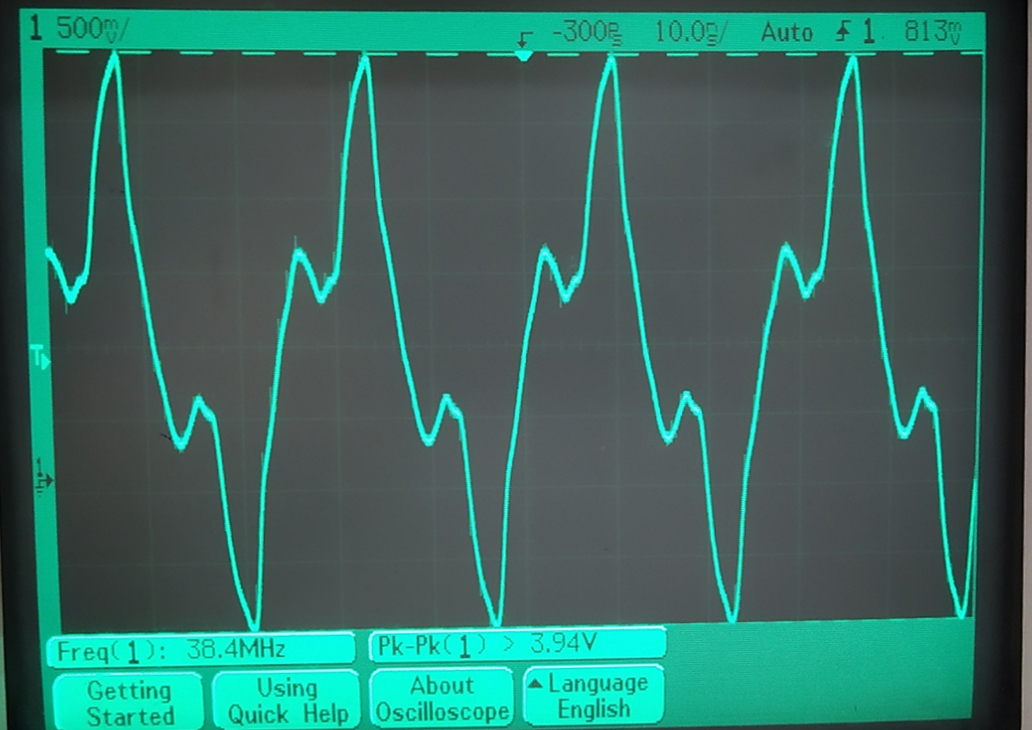
\includegraphics[width=0.7\linewidth]{figures/clk.jpg}
	\caption{Xung đồng hồ tham chiếu đầu ra của BladeRF}
	\label{fig:clk}
\end{figure}
\begin{figure} [!h]
	\centering
	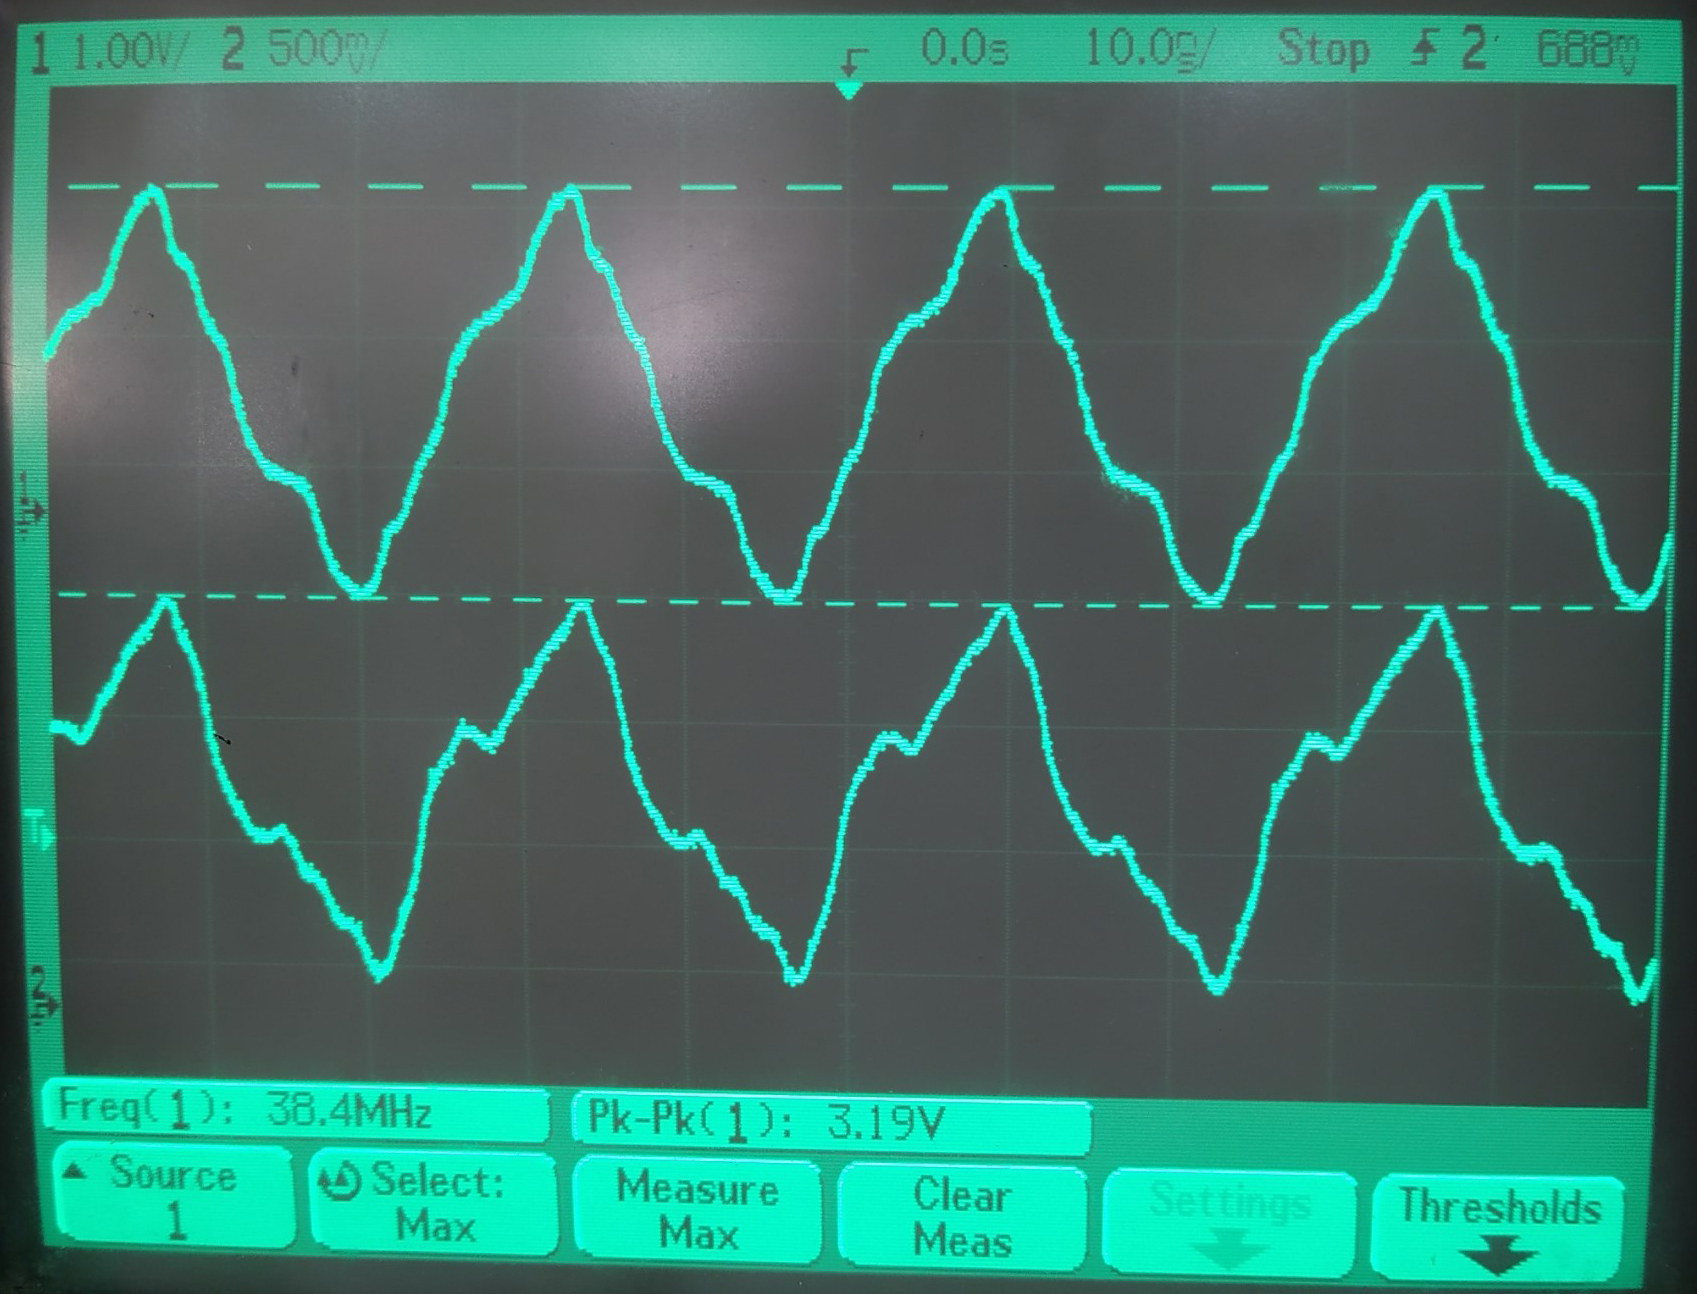
\includegraphics[width=0.7\linewidth]{figures/shareclk.jpg}
	\caption{Xung đồng hồ tham chiếu được chia sẻ}
	\label{fig:shareclk}
\end{figure}

\newpage

\begin{itemize}
	\item[$\ast$] \textbf{$\textbf{Hiệu chỉnh } \textbf{f}_{\textbf{offset}}$}
\end{itemize} 

$f_{\textrm{offset}}$ hay chính xác hơn là tần số sóng mang offset CFO (Carrier Frequency Offset), luôn tồn tại khi LO (Local Oscillator) chịu ảnh hưởng bởi nhiễu điện, chênh lệnh nhiệt độ, ... Những độ lệch này có thể tạo ra $f_{\textrm{offset}}$ và $\textrm{phase}_\textrm{offset}$ ngẫu nhiên. Trên các SDR thương mại, các thông số này đã được tính toán, và được bù lại bởi VCTCXO với độ chính xác biểu thị bởi thông số PPM (Parts Per Million). Ví dụ như BladeRF được cân chỉnh ở mức 1 PPM ở nhà máy thì $f_{\textrm{offset}}$ tối đa nếu phát/thu tín hiệu ở tần số sóng mang 923 MHz tương đương:
\begin{equation}
f_{\mathrm{offset  max}} = \frac{f_c \times\textrm{ PPM}}{10^6} = \frac{923\times 10^6 \times 1}{10^6} = 923 \textrm{ Hz}
\end{equation}

923 Hz là khá lớn, để giảm đi sai số này, nhà sản xuất cung cấp công cụ kalibrate-bladeRF \cite{kali}, cho phép người dùng sử dụng tín hiệu từ 1 kênh FCCH (Frequency Correction Channel) đường xuống từ trạm cơ sở GSM ở gần để hiệu chỉnh lại VCTCXO có thể xuống mức 0,014 PPM, tương đương với việc sai số 923 Hz như trên có thể giảm xuống 10 Hz. Kết quả thực tế như trên hình \ref{fig:freqcal} và \ref{fig:freqanly}, sau khi hiệu chỉnh kết quả thu được sai số chỉ 5 Hz ở 923 MHz và độ lệch $\Delta f_{\mathrm{offset}} = 20\textrm{ Hz}$.
\begin{figure} [!h]
	\centering
	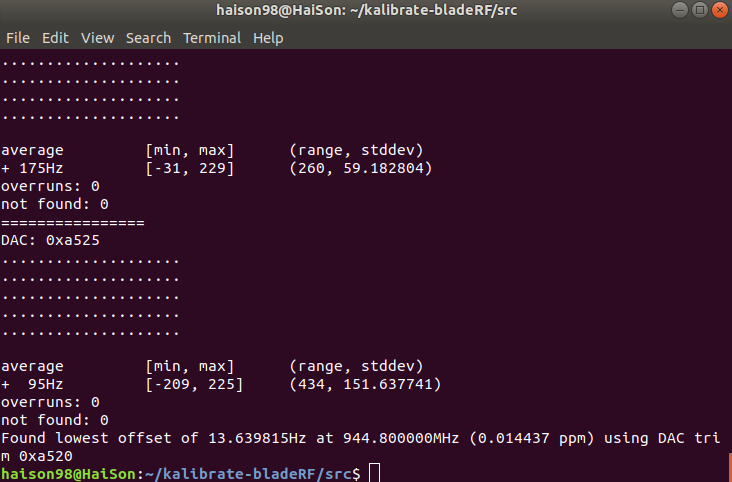
\includegraphics[width=0.85\linewidth]{figures/freqcal.png}
	\caption{Kết quả cân chỉnh tần số với kalibrate-bladeRF}
	\label{fig:freqcal}
\end{figure}

%Ngoài phương pháp sử dụng phần mềm, BladeRFx115 cung cấp cổng J71 pin 1 để người dùng sử dụng máy phát tín hiệu chuyên dụng tự hiệu chỉnh VCTCXO bằng tín hiệu 1 xung/giây, hoặc 10 MHz ở mức điện áp 1,8 V.

\begin{figure} [!ht]
	\centering
	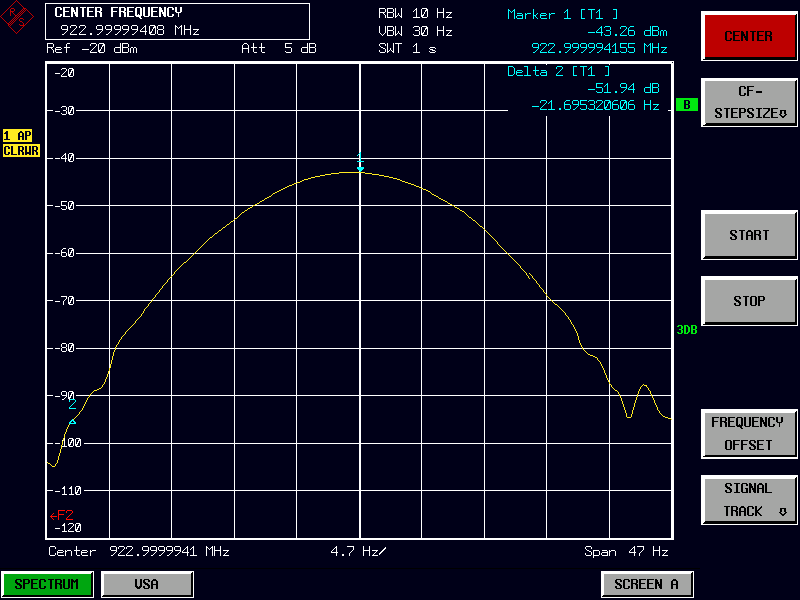
\includegraphics[width=0.85\linewidth]{figures/freqanly.png}
	\caption{Kết quả thu được trên máy phân tích phổ}
	\label{fig:freqanly}
\end{figure}

\begin{itemize}
	\item[$\ast$] \textbf{Hiệu chỉnh $\textbf{DC}_{\textbf{offset}}$ và cân bằng  mẫu IQ}
\end{itemize}

 Do được thiết kế như một bộ nhận chuyển đổi trực tiếp (Direct-conversion receiver) hay bộ nhận không có tần số trung gian (zero-IF receiver) nên trong kết quả mẫu đầu ra từ BladeRF, khi được đưa lên phổ FFT, sẽ luôn có một đỉnh phổ ở tần số trung tâm 0 Hz biểu diễn cho điện áp DC, hiện tại BladeRF chưa có phần cứng để bù vào phần DC này nên chỉ có thể giảm thiểu về mức thấp.

Nhà sản xuất đã tích hợp sẵn việc hiệu chỉnh trong thư viện của BladeRF, chi tiết có tại \cite{Dccali}. Ngoài việc hiệu chỉnh trên phần cứng BladeRF, cần sử dụng thêm khối DC Blocker trên GNU Radio để loại bỏ hoàn toàn thành phần DC.

\begin{itemize}
	\item[$\ast$] \textbf{Hiệu chỉnh $\textrm{sample}_{\textbf{offset}}$}
\end{itemize} 

Trong khóa luận này sẽ sử dụng tương quan chéo của tín hiệu thu để ước lượng số mẫu trễ gây ra bởi phần cứng BladeRF và USB. Đây là phương pháp có tính linh hoạt cao, có thể đồng bộ lượng mẫu đầu vào lớn (chục triệu mẫu), tuy nhiên bị giới hạn độ chính xác bởi môi trường truyền.

Tương quan chéo biểu hiện cho sự giống nhau của 2 tín hiệu, trong trường hợp này, có thể được dùng để ước lượng trễ mẫu giữa tín hiệu thu được từ 2 BladeRF bằng việc sử dụng một tín hiệu tham chiếu $\mathbf{x}(t)$. Trước hết, công thức toán học của tương quan chéo được ký hiệu $\mathbf{x_1 \star x_2}$ giữa 2 tín hiệu phức \cite{Bracewell1978}:
\begin{equation}
\begin{split}
&\mathbf{x}(t): \textrm{Tín hiệu cơ sở}\\
&\mathbf{x}_1(t) =\mathbf{x}(t)\\
&\mathbf{x}_2(t) =\mathbf{x}(t - T) \\
&\mathbf{x_1 \star x_2}(\tau) \triangleq \int_{-\infty}^{+\infty} \mathbf{x}_{1}^{*} (t) \mathbf{x}_{2} (t + \tau) dt \\
&T =\textrm{argmax}(\mathbf{x_1 \star x_2})
\end{split}
\end{equation}
với $^*$ là ký hiệu của liên hợp phức, chỉ có nghĩa khi $\mathbf{x}_1$ là số phức, $T$  là thời gian trễ giữa 2 tín hiệu. Rời rạc công thức tương quan chéo (2.2) để áp dụng cho các mẫu:
\begin{equation}
\mathbf{x_1 \star x_2}(n) = \sum_{m = -\infty}^{\infty} \mathbf{x}^*_1 (m) .\mathbf{x}_2 (m + n)
\end{equation}
tương tự thì số mẫu trễ tương ứng là $n = \mathrm{argmax(\mathbf{x_1 \star x_2})}$. Trên hình \ref{fig:xcorr} là ví dụ về việc sử dụng tương quan chéo của nhiễu Gauss để tìm độ trễ mẫu do phần cứng gây ra, được mô phỏng là 100 mẫu. 
\begin{figure} [!h]
	\centering
	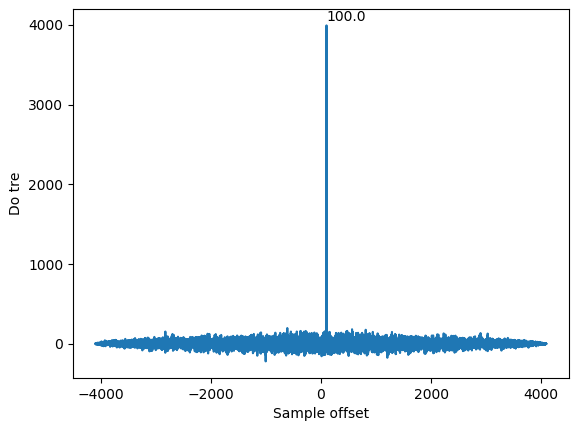
\includegraphics[width=0.8\linewidth]{figures/xcorr.png}
	\caption{Tương quan chéo của 2 nhiễu Gauss}
	\label{fig:xcorr}
\end{figure}

Cũng sử dụng tính tương quan của tín hiệu để tìm độ trễ, tuy nhiên thay vì tính toán ngay trên miền thời gian, việc chuyển sang miền tần số sẽ giúp giảm đáng kể lượng tính toán cần thiết do sử dụng khối FFT trên GNU Radio hỗ trợ chia đa luồng xử lý. Sử dụng các phép biến đổi  FFT, IFFT để tính toán trễ giữa hai tín hiệu \cite{Nentwig2016}. Áp dụng trên GNU Radio, với các khối có sẵn FFT, IFFT, Multipy Conjugate, dữ liệu đầu vào là tín hiệu được điều chế tần số băng hẹp (Narrow band FM - NBFM) được chia thành 2 nguồn, nguồn đầu tiên bị trễ 1000 mẫu so với nguồn thứ 2, lưu đồ tương ứng trên GNU Radio như hình \ref{fig:fft} và kết quả đầu ra biểu diễn qua QT GUI trên hình \ref{fig:dvb-t2} với vị trí đỉnh phổ đúng bằng số lượng trễ mô phỏng.
\begin{equation}
\begin{split}
&\mathbf{x}_1(t) \Leftrightarrow \mathbf{x}_1(f)\\
&\mathbf{x}_2(t) \Leftrightarrow \mathbf{x}_2(f)\\
&\mathbf{x_1 \star x_2} (\tau) \Leftrightarrow \mathbf{x_1 \star x_2}(f)\\
&\mathbf{x_1 \star x_2}(f) = \mathbf{x}_1^{*}(f) \mathbf{x}_2(f)
\end{split}
\end{equation}
\begin{figure}[!h]
%\hfill
\centering
\subfigure[Flow-graph mô phỏng ước lượng độ trễ giữa các đầu vào]{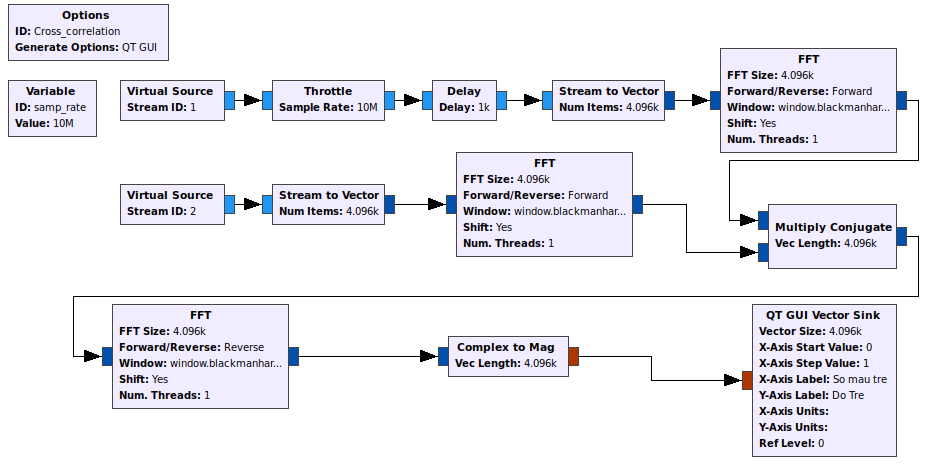
\includegraphics[width=1\linewidth]{figures/fft.png}\label{fig:fft}}
\hfill
\subfigure[Tương quan chéo của tín hiệu đầu vào]{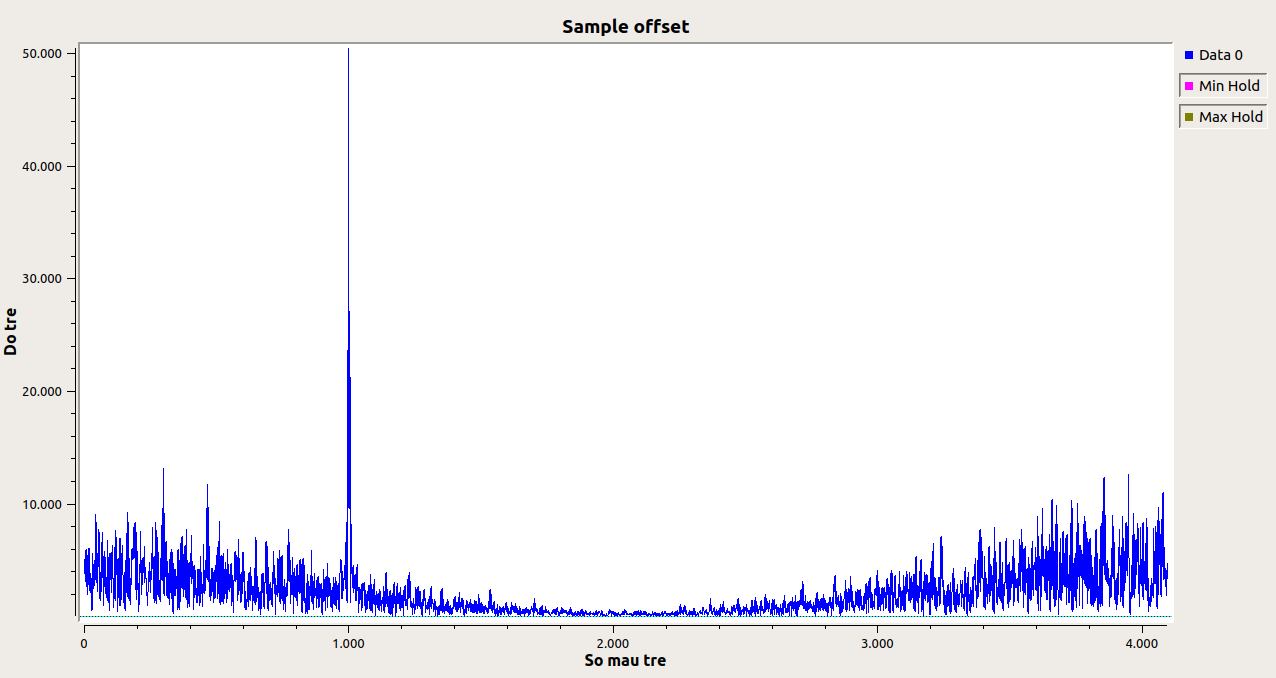
\includegraphics[width=1\linewidth]{figures/dvb-t2.png}\label{fig:dvb-t2}}
\hfill
\caption{Xác định độ trễ mẫu trên GNU Radio}
\end{figure}

Sau khi đã xác định được số mẫu trễ, sử dụng khối Delay, trễ mẫu của khối nguồn đang chạy nhanh đi một lượng $\mathrm{argmax[\mathbf{x_1 \star x_2}(f)]}$.  Flow-graph \ref{fig:fft} được viết gọn vào một khối duy nhất Sample Offset như hình \ref{fig:sample_offset} để tiện cho việc xử lý, $\textrm{sample}_\textrm{offset}$ được lưu vào một biến và phản hồi lại về đầu vào để  căn chỉnh dữ liệu khớp với nhau về mặt thời gian sẵn sàng cho các  khối xử lý tiếp theo trong GNU Radio.

\begin{figure}[!h]
%\hfill
\subfigure[Ước lượng $\textrm{sample}_\textrm{offset}$ ]{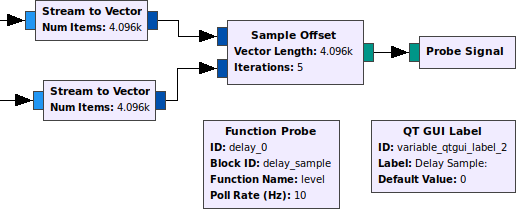
\includegraphics[width=0.6\linewidth]{figures/sample_offset.png}}
\hfill
\subfigure[Phản hồi  $\textrm{sample}_\textrm{offset}$]{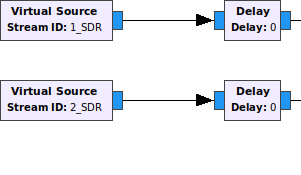
\includegraphics[width=0.35\linewidth]{figures/sample_offset_fb.png}}
\hfill
\caption{Ước lượng và phản hồi hiệu chỉnh $\textrm{sample}_\textrm{offset}$}
\label{fig:sample_offset}
\end{figure}

Nhược điểm của phương pháp này: nếu tín hiệu đầu vào có tính tương quan cao, kết quả đầu ra sẽ không chính xác tùy thuộc vào sự tương quan đó, mô phỏng cùng với kết quả mô phỏng của vấn đề này được trình bày trong mục 3.1.2 tại bảng 3.1 và 3.2; nếu độ trễ mẫu quá lớn, thông thường lớn hơn 1/2 số mẫu đầu vào khối FFT thì không thể tìm được độ trễ của các nguồn. Vì vậy, số lượng phần tử được đưa vào FFT có thể nâng lên đến hàng trăm nghìn phần tử để chắc chắn rằng thu được độ trễ khớp, nhưng để giảm thiểu tính toán, chỉ cần thực hiện hiệu chỉnh $\textrm{sample}_\textrm{offset}$ ngay khi hệ thống khởi động và lưu giá trị trễ cố định cho toàn bộ thời gian chương trình chạy. Do một khi luồng dữ liệu từ SDR đã vào được GNU Radio, lượng trễ này sẽ giữ ở mức ổn định.

\begin{itemize}
	\item[$\ast$] \textbf{$\textbf{Hiệu chỉnh } \textbf{phase}_\textbf{offset}$}
\end{itemize} 

Tiếp đến là căn chỉnh lại pha giữa các SDR, sao cho tất cả pha từ dữ liệu là thẳng hàng trước khi ước lượng DOA, điều này là bắt buộc ngay cả khi cố định xung lấy mẫu qua chân J71-4, do việc hiệu chỉnh $\textrm{sample}_\textrm{offset}$ chỉ có độ phân giải nhỏ nhất một mẫu, và sự sai khác nhỏ hơn một mẫu chính là sai khác pha ban đầu. 

Sử dụng một tín hiệu tham chiếu bên ngoài đặt ở góc 90$^{\circ}$ để căn chỉnh pha, do được truyền qua kênh truyền với nhiễu, đa đường, suy giảm,... nếu ước lượng sai khác pha trực tiếp: $\Delta \phi = \phi_1 - \phi_0$, sự sai khác pha tính toán ra sẽ phát sinh những sai số ngẫu nhiên khó để căn chỉnh chính xác pha về trạng thái cân bằng. Vì vậy, dưới đây là phương pháp sử dụng ngay thuật MUSIC toán ước lượng DOA để tính toán ra độ lệch pha giữa các tín hiệu.

Căn chỉnh $\textrm{phase}_\textrm{offset}$ trên GNU Radio, để đảm bảo pha ban đầu trên các SDR như nhau, sử dụng một tín hiệu bên ngoài là nguồn tham chiếu, đặt tín hiệu ở góc 90$^{\circ}$. Sau khi hiệu chỉnh được $\textrm{sample}_\textrm{offset}$ như ở  phần trước. Tín hiệu thu được sẽ tồn tại độ lệch pha ($\textrm{phase}_\textrm{offset}$), các bước chính để căn chỉnh:
\begin{itemize}
	\item Tính toán ma trận hiệp phương sai $\mathbf{R}_\mathbf{x}$ của các tín hiệu.
	\item Tìm 2 ma trận giá trị riêng ($\mathbf{\Lambda}$) và vector riêng ($\mathbf{E}$) từ ma trận hiệp phương sai.
	\item Ước lượng sự sai khác pha của SDR bằng thuật toán MUSIC \cite{Whiting2018}.
	\item Phản hồi sai khác pha về một khối Multipy Exp (hay $e^{j\Delta\phi}$).
	\item Căn chỉnh liên tục đến ngưỡng cân bằng khi phương sai giảm xuống thấp.
	\item Chuyển đổi hệ từ trạng thái đồng bộ sang ước lượng DOA.
\end{itemize}

Tất cả các bước được gộp thành 3 khối PCA Phase Diff, Hold và Multipy Exp, lưu đồ của hiệu chỉnh như hình \ref{fig:phasediff}.

\begin{figure} [!ht]
	\centering
	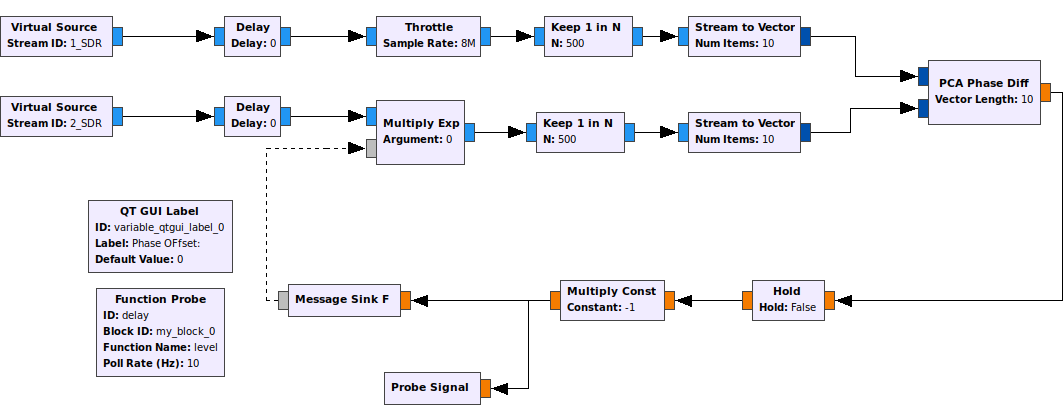
\includegraphics[width=1\linewidth]{figures/phasediff.png}
	\caption{Ước lượng và phản hồi $\textrm{phase}_\textrm{offset}$}
	\label{fig:phasediff}
\end{figure}

Kết quả thực nghiệm trên hình 2.18, khi phát NBFM ở tần số 923 MHz trên 1 BladeRF, 2 BladeRF thu, tính toán $\textrm{sample}_\textrm{offset}$ và căn chỉnh pha.
\afterpage{\clearpage}
\begin{figure}[!ht]
%\hfill
\centering
\subfigure[Tín hiệu ban đầu chưa đồng bộ]{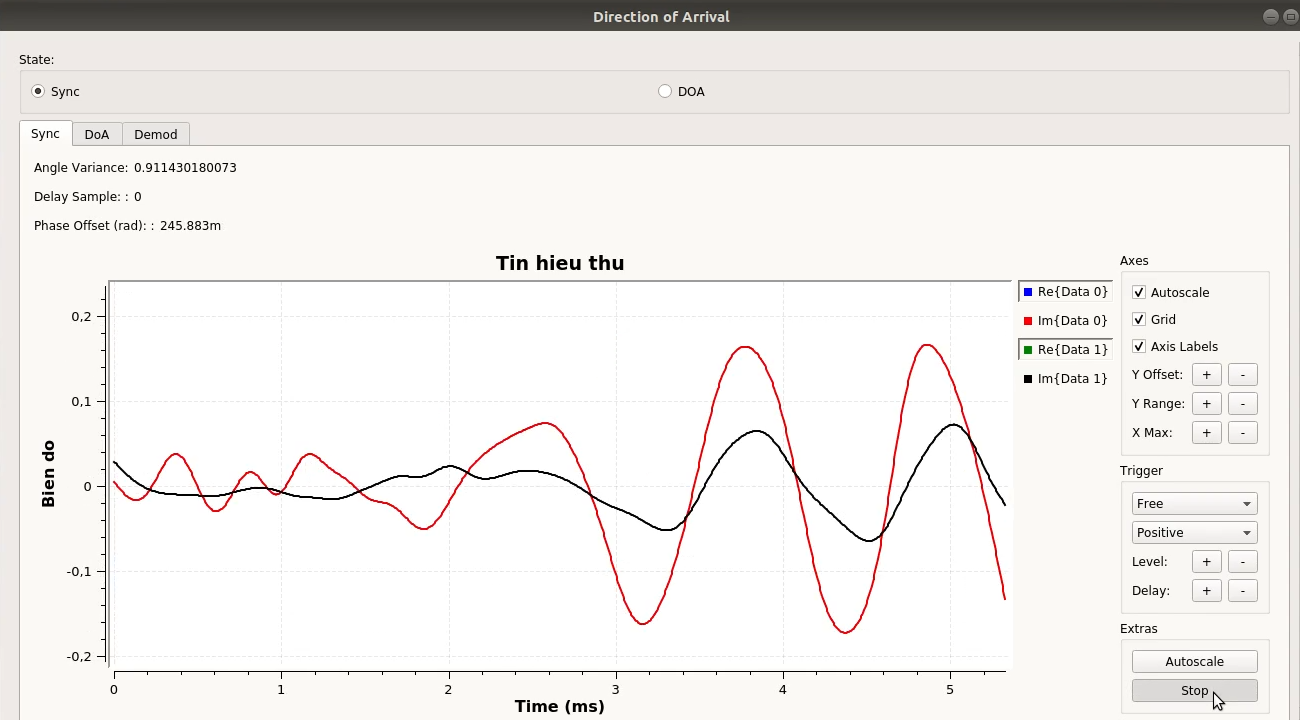
\includegraphics[width=0.8\linewidth]{figures/nonshift.png}\label{fig:nonshift}}
\hfill
\subfigure[Tín hiệu sau khi dịch mẫu và căn chỉnh pha]{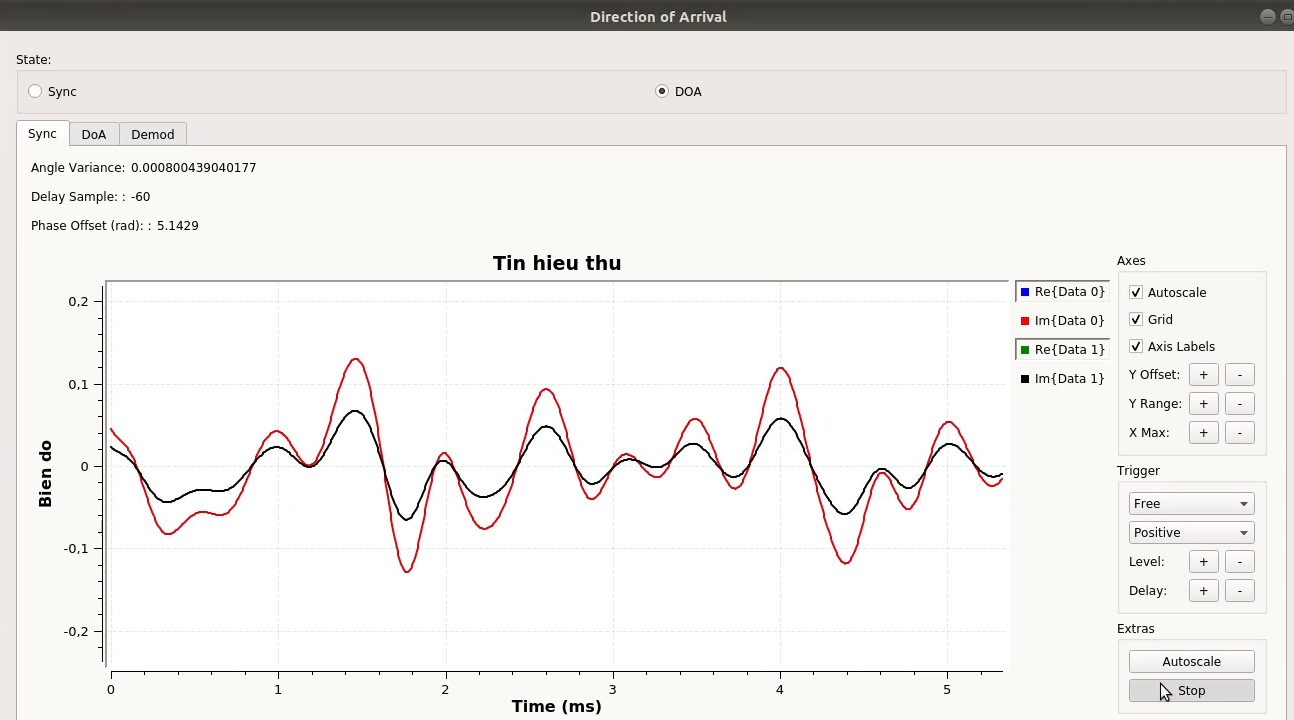
\includegraphics[width=0.8\linewidth]{figures/shifted.png}\label{fig:shifted}}
\hfill
\subfigure[Góc đầu ra ban đầu khi hệ được đồng bộ]{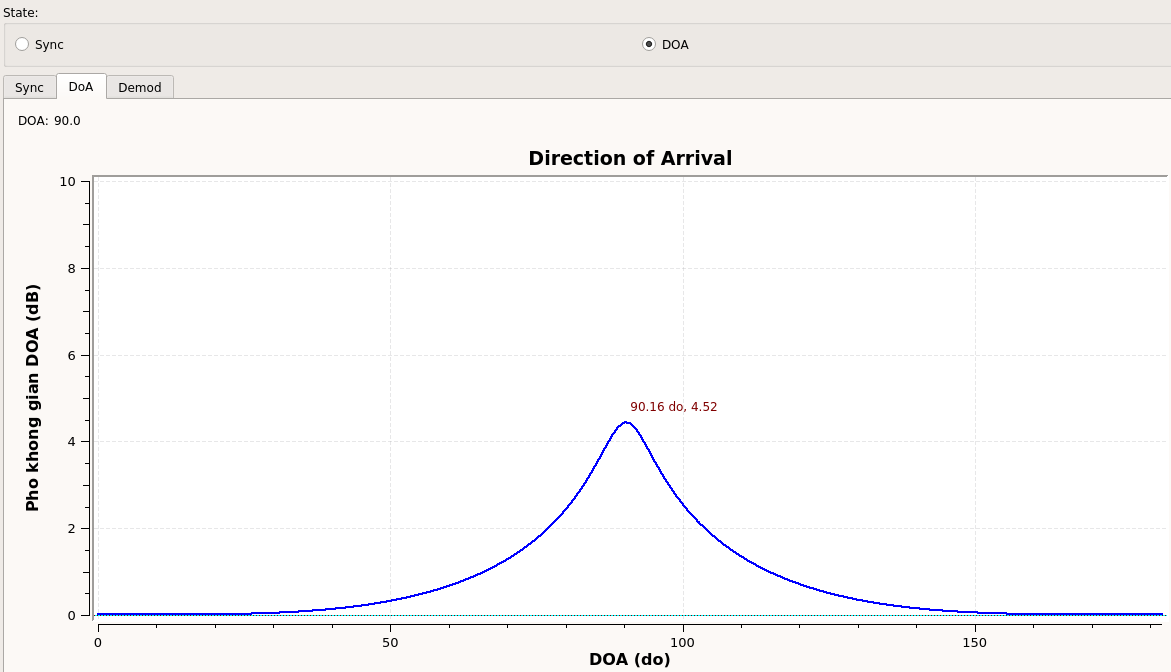
\includegraphics[width=0.8\linewidth]{figures/DOA_sync.png}
\hfill
\label{fig:DOA_sync}}
\caption{Kết quả đồng bộ hệ SDR}
\end{figure}